\documentclass{acm_proc_article-sp}
\usepackage{url}
\usepackage{tikz}

\begin{document}
\title{Demo: Spectrum Agile mm-Wave Packet Radio}
%
% You need the command \numberofauthors to handle the 'placement
% and alignment' of the authors beneath the title.
%
% For aesthetic reasons, we recommend 'three authors at a time'
% i.e. three 'name/affiliation blocks' be placed beneath the title.
%
% NOTE: You are NOT restricted in how many 'rows' of
% "name/affiliations" may appear. We just ask that you restrict
% the number of 'columns' to three.
%
% Because of the available 'opening page real-estate'
% we ask you to refrain from putting more than six authors
% (two rows with three columns) beneath the article title.
% More than six makes the first-page appear very cluttered indeed.
%
% Use the \alignauthor commands to handle the names
% and affiliations for an 'aesthetic maximum' of six authors.
% Add names, affiliations, addresses for
% the seventh etc. author(s) as the argument for the
% \additionalauthors command.
% These 'additional authors' will be output/set for you
% without further effort on your part as the last section in
% the body of your article BEFORE References or any Appendices.

\numberofauthors{1} %  in this sample file, there are a *total*
% of EIGHT authors. SIX appear on the 'first-page' (for formatting
% reasons) and the remaining two appear in the \additionalauthors section.
%
\author{
% You can go ahead and credit any number of authors here,
% e.g. one 'row of three' or two rows (consisting of one row of three
% and a second row of one, two or three).
%
% The command \alignauthor (no curly braces needed) should
% precede each author name, affiliation/snail-mail address and
% e-mail address. Additionally, tag each line of
% affiliation/address with \affaddr, and tag the
% e-mail address with \email.
%
% 1st. author
\alignauthor
Julian Arnold, Ljiljana Simi\'{c}, Marina Petrova, Petri M\"ah\"onen\\
       \affaddr{Institute for Networked Systems}\\
       \affaddr{RWTH Aachen University}\\
       \affaddr{Kackertstrasse 9, 52072 Aachen, Germany}\\
       \email{\{jua,lsi,mpe,pma\}@inets.rwth-aachen.de}
}

\date{\today}

\maketitle
\begin{abstract}
We are presenting a spectrum agile mm-Wave packet radio communication system for multimedia streaming purposes.
The proposed system operates in the 60 GHz 70 GHz and 80 GHz bands.
\end{abstract}

% A category with the (minimum) three required fields
%\category{H.4}{Information Systems Applications}{Miscellaneous}
%A category including the fourth, optional field follows...
%\category{D.2.8}{Software Engineering}{Metrics}[complexity measures, performance measures]

%\terms{Theory}

%\keywords{mm-Wave, SDR, USRP, GNURadio} % NOT required for Proceedings

\section{Introduction}
The proposed system can be seen in Figure \ref{fig:system}. The system uses two USRP \cite{ettus} software defined radios to generate and receive a signal at an intermediate frequency. Two up/down-converts are used to transfer the intermediate frequency into the mm-Wave band. It is worth mentioning that the system can be operated in the 60 GHz, 70 GHz and 80 GHz bands.
We use a host PC to generate the packetized signal stream at baseband using GNURadio \cite{gnuradio}. The intermediate frequency can be adjusted from 1.2 GHz up to 6 GHz which offers a large amount of available bandwidth and allows the system to be spectrum agile. Figure \ref{fig:block} shows a block level description of the whole signal chain.
During the demo session we will demonstrate the proposed system, showing its operation in several mm-Wave bands.
\begin{figure}
\center
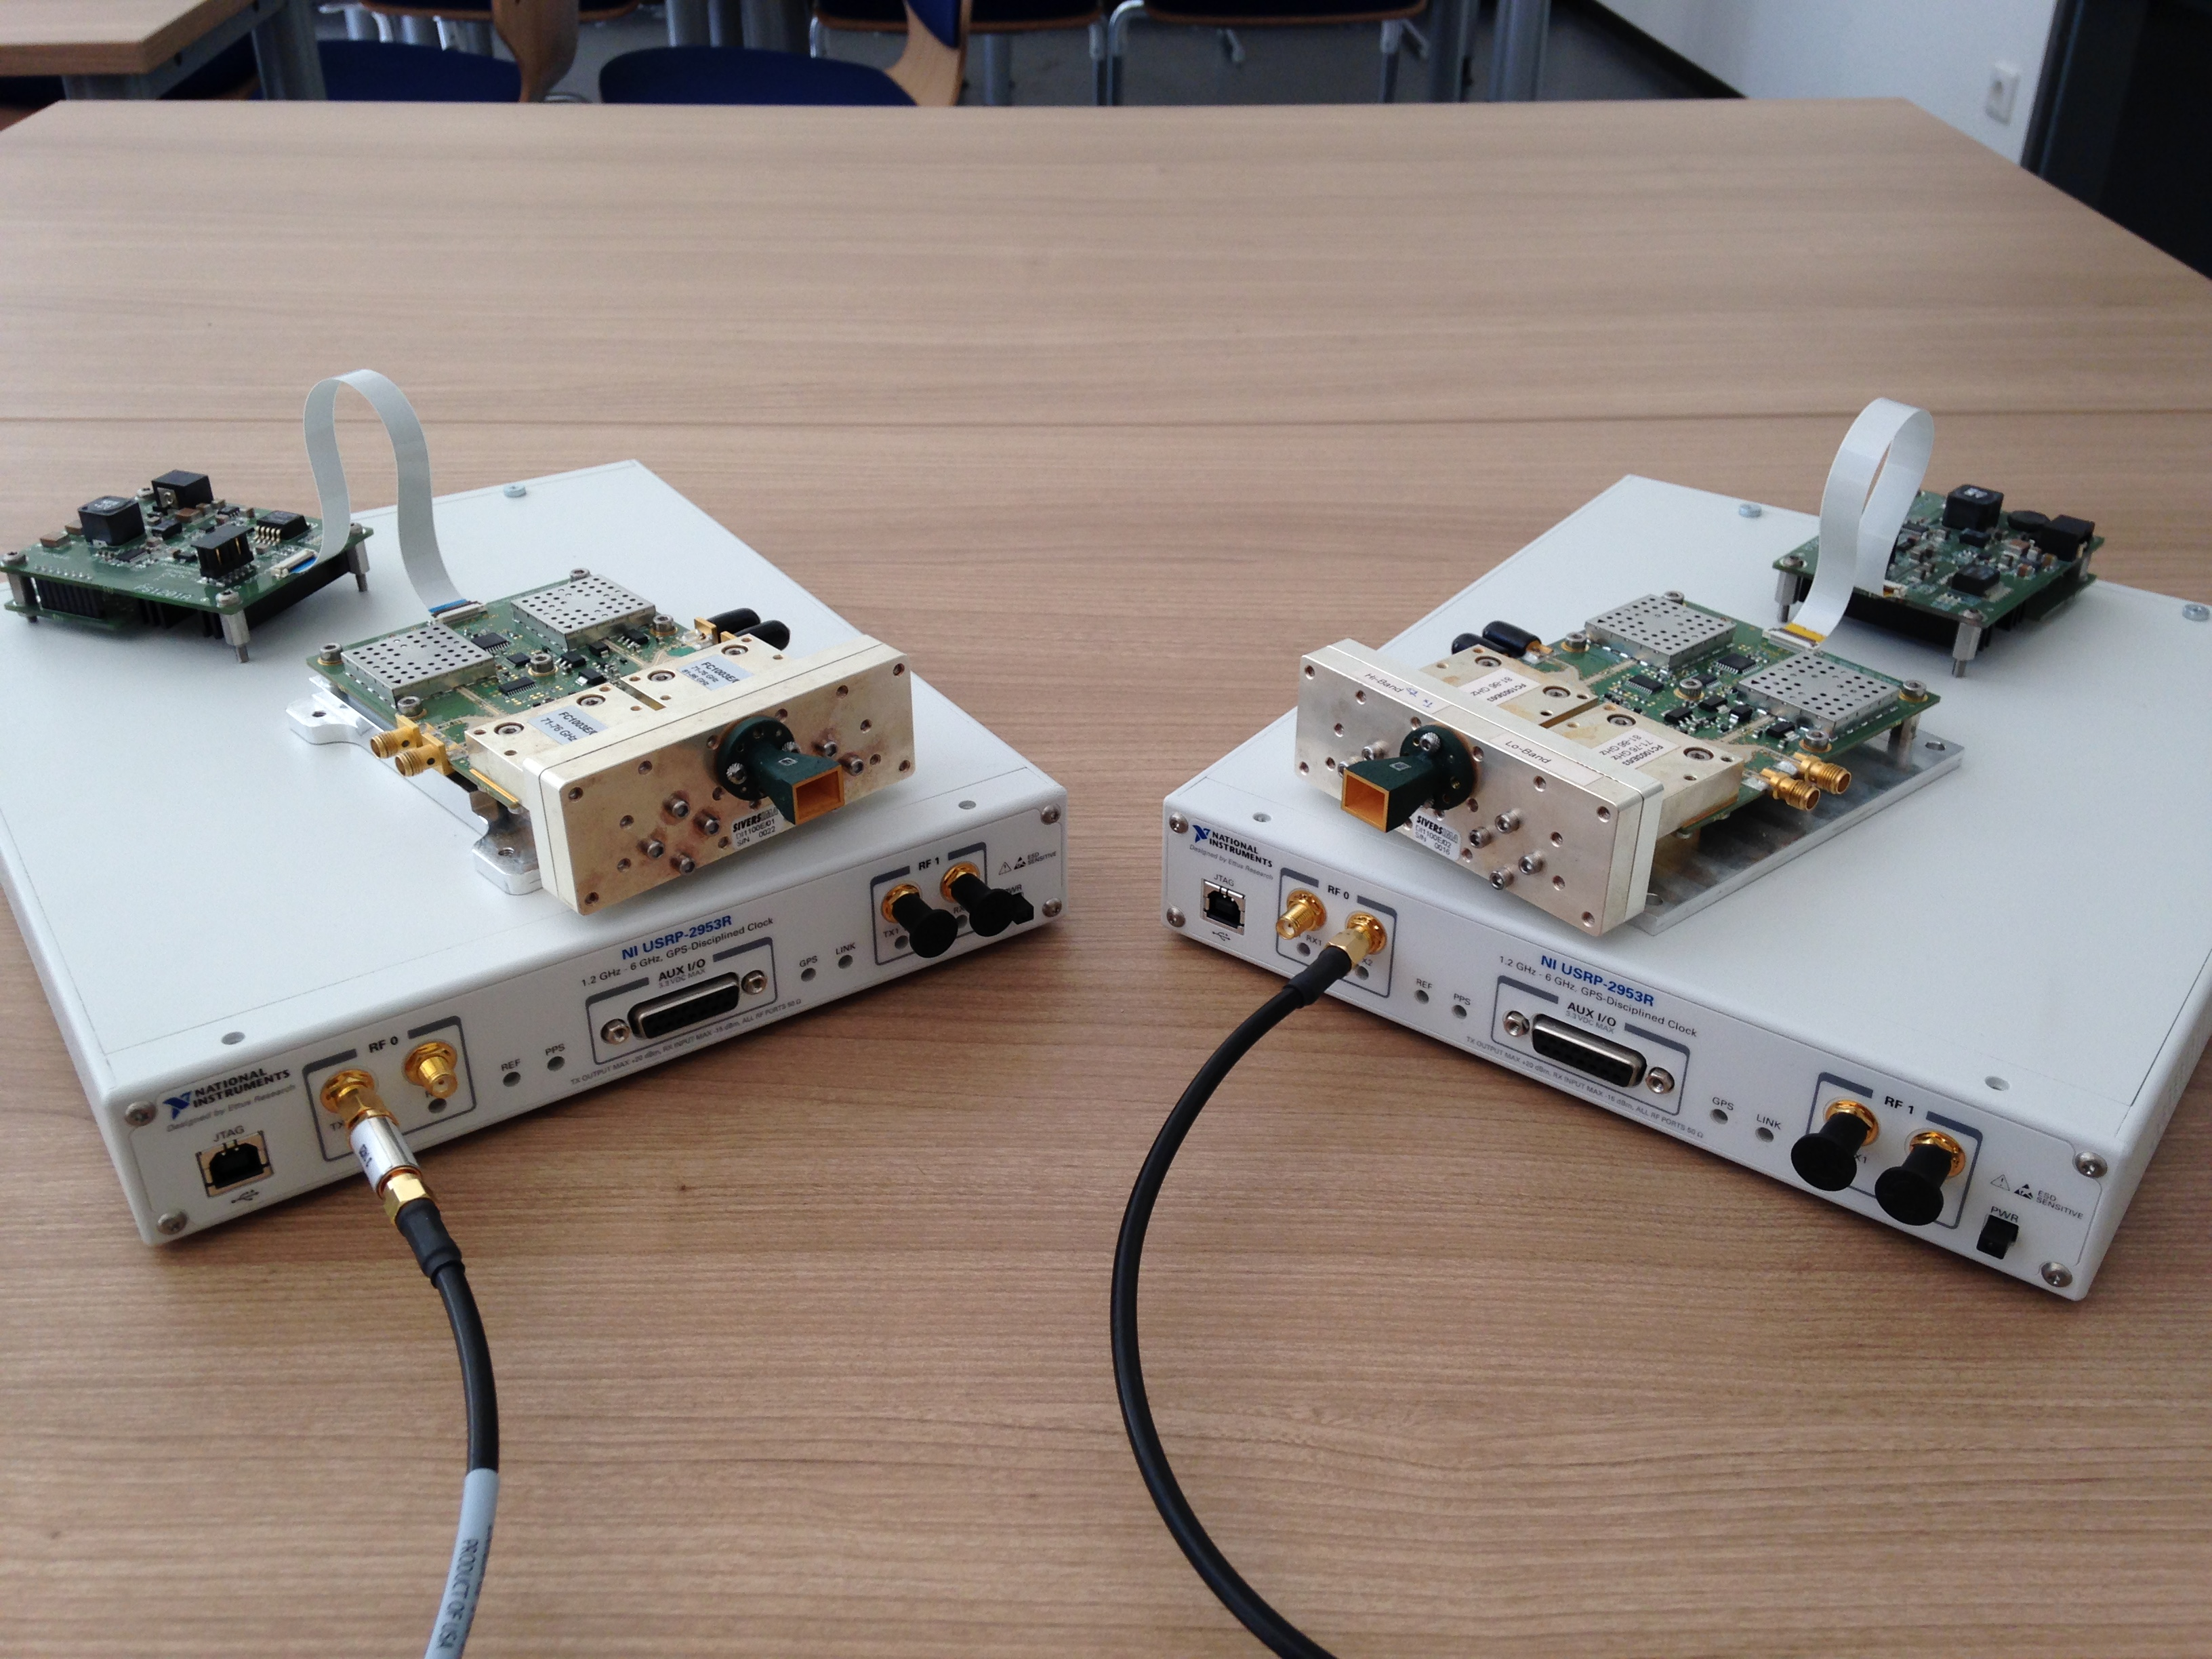
\includegraphics[width=0.4\textwidth]{system.jpg}
\caption{System Overview}
\label{fig:system}
\end{figure}
\begin{figure}
\center
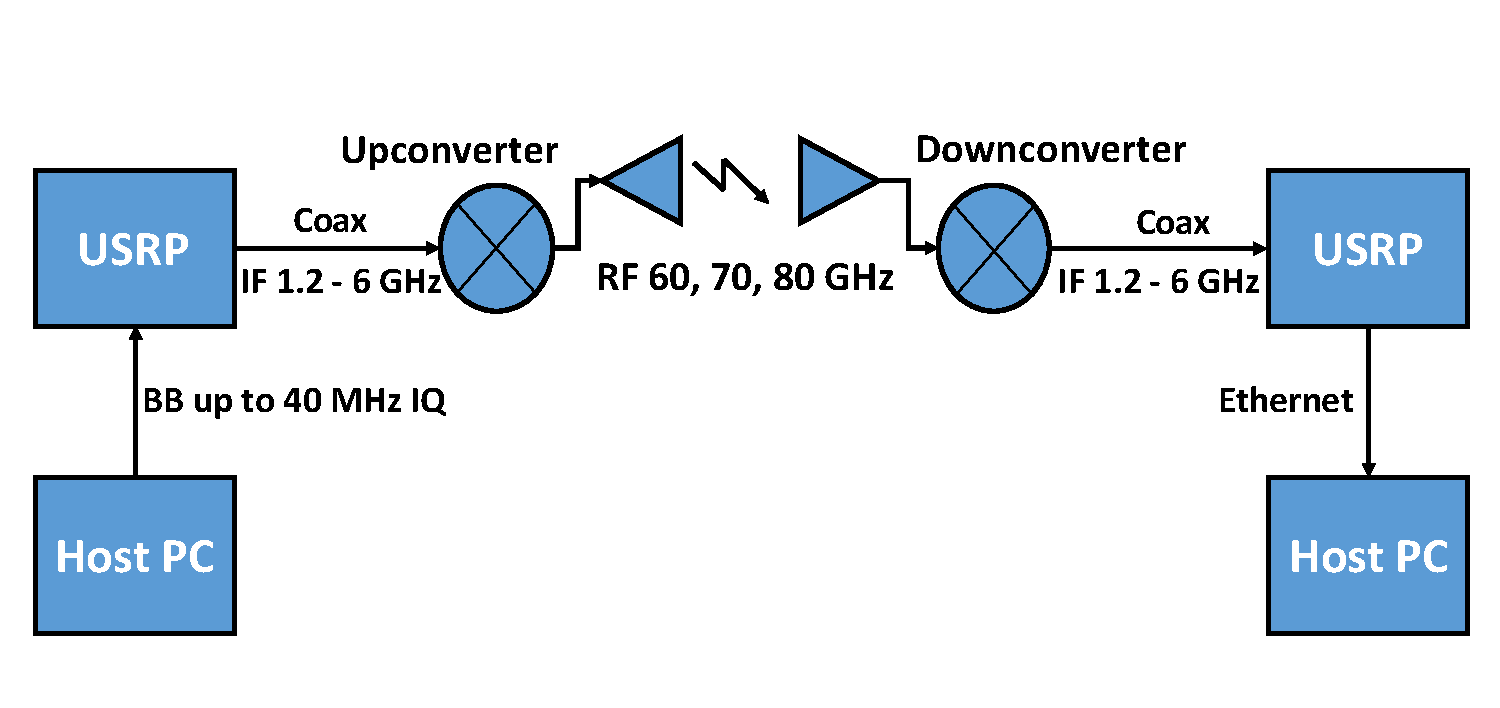
\includegraphics[width=0.4\textwidth]{block-diagram}
\caption{Block Level Description}
\label{fig:system}
\end{figure}
%\begin{figure}
%\begin{tikzpicture}
%\draw[thick] (0, 0) rectangle (1,1) node[pos=.5] {USRP};
%\draw[thick, ->] (1,.5) -- (2,.5);
%\draw[thick] (2.4, 0.5) -- (3,.5);
%\end{tikzpicture}
%\caption{Do not forget!
%Make it explicit enough that readers
%can figure out what you are doing.}
%\end{figure}

\bibliographystyle{abbrv}
\bibliography{sigproc}
\end{document}